\section{Appendix H - Air Sampling Model for BEXUS Flight}\label{sec:appH}


\subsection{Introduction}

% que es aixo? simulation software for ascent and Descent Phases

\subsubsection{Objectives}

The purpose of this is to theoretically simulate the experiment; its preparation, the sampling methodology, and the expected results.

\subsubsection{Justification}
% why?
% The air sample volume is limited, how it should be distributed over the altitude?
% How many bags do we need?
% When we will open and close each bag?
% How big the bags should be?
% many parameter changing over the altitude and time: gondola velocity, air pressure and density (required sampling volume), pump efficiency (sampling time)
% parameter to control: bags resolution (Tubular number??)

This theoretical model will give an estimation of the time needed to fill the bags in order to achieve the best resolution, the required volume of the samples at the different altitudes, to make sure that there is enough sample left for analysis, the sampling altitudes and the number of the bags.  

\subsubsection{Methodology}
% how?
% context study, critical scenarios identification, equations, matlab simulation, verification with empirical measures.

For this purpose, a mathematical model was created using MATLAB. In order to make sure that this model is reliable, it is going to be tested for the atmospheric conditions in the Arctic, and then compared with the 1976 US Standard atmosphere model that is used for this region. What is more, the model will be compared with past BEXUS flight data. The goal of the model is to be as close as possible with these past data. 
After the tests, and making sure that the mathematical model is accurate, it will be adjusted with the TUBULAR's experiment requirements. In this way, the team will get a general picture of the experiment's layout. Hence, the results of the experiment will be more or less expected, and in the case of complications, the mathematical model will be used as a reference of understanding what went wrong.


\subsection{Scientific and Empirical Background}

\subsubsection{Study of previous BEXUS flights}
This section has been elaborated based on the flight data files located in the previous BEXUS flights folders in the REXUS/BEXUS teamsite. This data was recorded by the Esrange Balloon Service System (EBASS).

\smallskip
This unit is responsible of the piloting of the balloon is done by Esrange. It provides the communication link between the gondola and the ground station. The EBASS airborne unit, receives the data from the on board sensors, and then it sends them to the EBASS ground unit. It is also responsible for the payload control, providing functions like the altitude control, by valve and ballast release or the flight termination. What is more, EBASS keeps track of the filght trajectory with an on-board GPS system.

\smallskip
Tables \ref{table:pre-flight} and \ref{table:post-flight} below gather some general information before and after the BEXUS flights. The pre-flight and the post-flight data are more or less in agreement in estimating for example, the ascent/descent time, the cut-off altitude and the float time. Knowing those information and that the estimations are close enough to the real data, will help the team to define the experiment's parameters with higher accuracy. 

\smallskip
It is worth mentioning that the ascent speed in Table \ref{table:post-flight} is lower than the predicted $5\sim 6 m/s$ which is mentioned in the BEXUS manual. That is because it is the average velocity value of all the data points.  

\begin{table}[H]

\noindent\makebox[\columnwidth]{%
\scalebox{0.8}{
\begin{tabular}{c|c|c|c|c|c|c|}
\cline{2-7}
\multicolumn{1}{l|}{} & \textbf{BEXUS 20} & \textbf{BEXUS 21} & \textbf{BEXUS 22} & \textbf{BEXUS 23} & \textbf{BEXUS 24} & \textbf{BEXUS 25} \\ \hline
\multicolumn{1}{|c|}{Main Balloon} & Zodiac 12SF & Zodiac 12SF & Zodiac 35SF & Zodiac 35SF & Zodiac 12SF & Zodiac 12SF \\ \hline
\multicolumn{1}{|c|}{Balloon mass {[}kg{]}} & 101.4 & 101.4 & - & - & 101.4 & 101.4 \\ \hline
\multicolumn{1}{|c|}{Parachute {[$m^2$]}} & 80 & 80 & 80 & 80 & 80 & 80 \\ \hline
\multicolumn{1}{|c|}{Vehicle mass - Launch {[}kg{]}} & 256.8 & 287.8 & - & - & 300.6 & 321.15 \\ \hline
\multicolumn{1}{|c|}{Vehicle mass - Descent {[}kg{]}} & 155.4 & 186.4 & 189.58 & 181.5 & 199.2 & 219.75 \\ \hline
\multicolumn{1}{|c|}{Float altitude estimation {[}km{]}} & 28.2 & 27.5 & - & - & 27 & 26.6 \\ \hline
\multicolumn{1}{|c|}{Float pressure estimation {[}mbar{]}} & 15.38 & 17.11 & - & - & 18.5 & 19.6 \\ \hline
\multicolumn{1}{|c|}{Float temperature estimation {[}\degree C{]}} & - 48 & - 48 & - & - & - 49.5 & - 49.9 \\ \hline
\multicolumn{1}{|c|}{Estimated ascent time} & 1h 33min & 1h 31min & - & - & 1h 29min & 1h 27min \\ \hline
\end{tabular}}}
\caption{Pre-flight Information Available in Previous BEXUS Campaigns}
\label{table:pre-flight}
\end{table}


\begin{table}[H]

\noindent\makebox[\columnwidth]{%
\scalebox{0.8}{
\begin{tabular}{c|c|c|c|c|c|c|}
\cline{2-7}
 & \textbf{BEXUS 20} & \textbf{BEXUS 21} & \textbf{BEXUS 22} & \textbf{BEXUS 23} & \textbf{BEXUS 24} & \textbf{BEXUS 25} \\ \hline
\multicolumn{1}{|c|}{Ascent time} & 1h 37min & 1h 37min & 1h 51min & 1h 51min & 1h 55min & 3h 45min \\ \hline
\multicolumn{1}{|c|}{Average ascent speed [m/s]} & 4.78 & 4.59 & 4.52 & 4.79 & 3.79 & 1.86 \\ \hline
\multicolumn{1}{|c|}{Floating altitude [km]} & 28 & 27 & 32 & 32 & 26.5 & 25.8 \\ \hline
\multicolumn{1}{|c|}{Floating time} & 2h 10min & 1h 46min & 2h 34min & 2h 42min & 2h 9min & 2h 36min \\ \hline
\multicolumn{1}{|c|}{Cut-off altitude [km]} & 27.7 & 20.5 & 28 & 32 & 25.7 & 25.2 \\ \hline
\multicolumn{1}{|c|}{Ending altitude [m]} & 648 & 723 & 3380 & 1630 & 1050 & - \\ \hline
\multicolumn{1}{|c|}{Descent time} & 36 min & 31 min & 29 min & 31 min & 30 min & - \\ \hline
\end{tabular}}}
\caption{Post-flight Information Regarding the Flight Profile for Previous BEXUS Campaings} \label{table:post-flight}
\end{table}

In order to find out how many bags it is possible to sample during ascent and Descent Phase it is important to know the time duration of each phase i.e Ascent, Floating and Descent. For that reason, Figure \ref{fig:trajectories} provides some sights on how previous BEXUS flights perform and what we can expect from BEXUS 26.

\begin{figure}[H]
    \begin{align*}
    \noindent\makebox[\textwidth]{%
        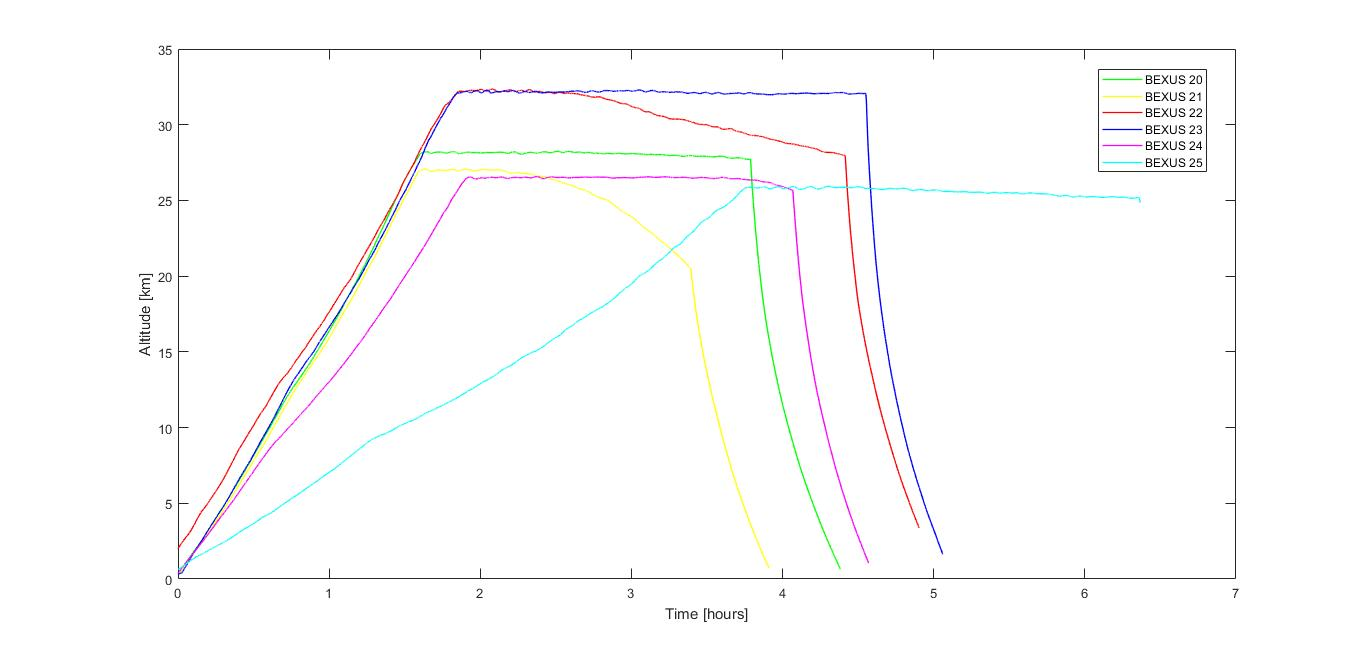
\includegraphics[width=1.2\textwidth]{appendix/img/flighttrajectory.png}}
    \end{align*}
    \caption{Altitude Over Flight Time for BEXUS Flights 20,21,22,23,24 and 25}\label{fig:trajectories}
\end{figure}

%\subsubsubsection{Gondola Dynamics}
\textbf{Gondola Dynamics}

The velocity of the gondola at each phase can give us information about its dynamics. For example, the data from the BEXUS flight 22 was chosen for analysis in order to get an idea of the velocity values and fluctuations throughout the flight. The obtained diagrams, with some marked points showing the time it takes for the gondola to reach a certain altitude, or the velocity of the gondola at a specific altitude, are shown below.   

\begin{figure}[H]
    \begin{align*}
    \noindent\makebox[\textwidth]{%
        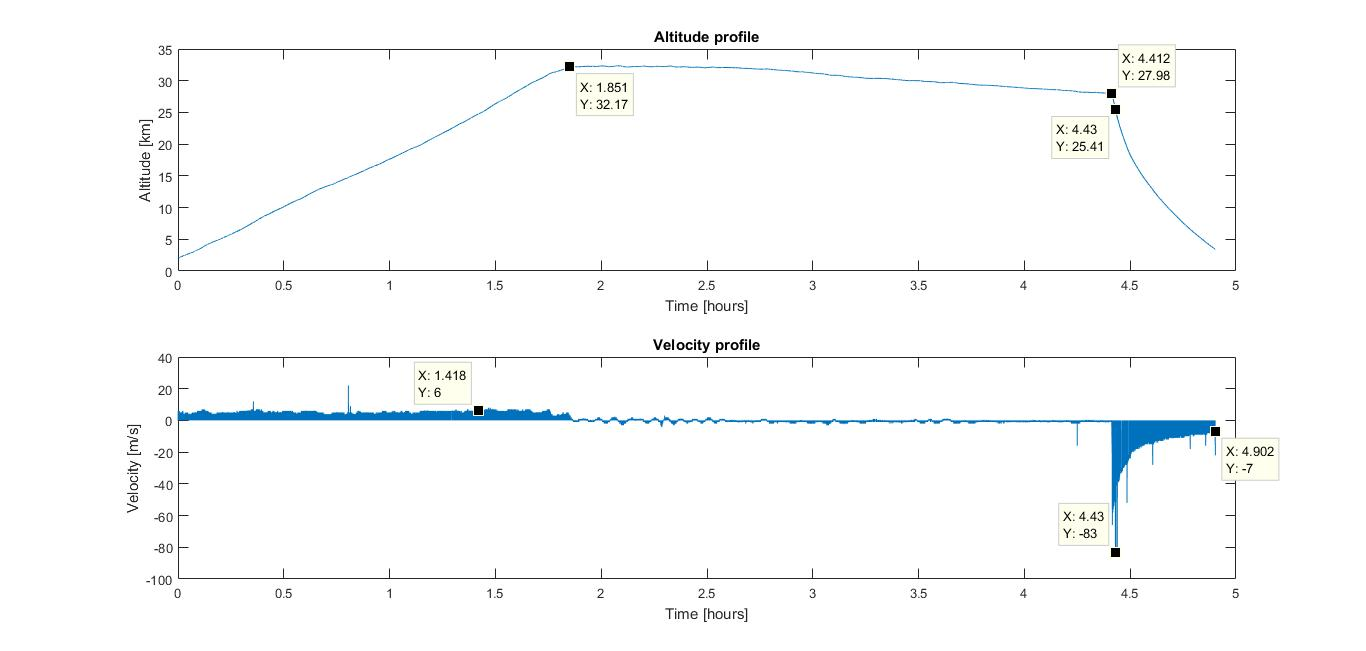
\includegraphics[width=1.2\textwidth]{appendix/img/altitudevelocity.png}}
    \end{align*}
    \caption{Altitude Profile [up] and Vertical Velocity Profile [down] Over the Flight Time During BEXUS 22 Flight}\label{fig:altitudevelocity}
\end{figure}

Figure \ref{fig:velocity} below, illustrates the velocity changes throughout the different phases.It works like a combination of both graphics form previous Figure \ref{fig:altitudevelocity}, however it provides a better representation of the velocity values at each phase. Specially during the Descent Phase, which is the most determinant for the air sampling process.

\smallskip
For each altitude, there are two velocity values, one for the Ascent and one for the Descent Phase. Constant and positive velocities indicate the Ascent Phase. During Ascent Phase the velocity is 6 m/s and almost constant, in agreement with the ascent speed value in the BEXUS manual. A zero velocity value indicates the Float Phase. Then the velocity becomes negative which indicates the Descent Phase. Once again, the velocity value close to the ground is 8 m/s as mentioned in the BEXUS manual.

\begin{figure}[H]
    \begin{align*}
    \noindent\makebox[\textwidth]{%
        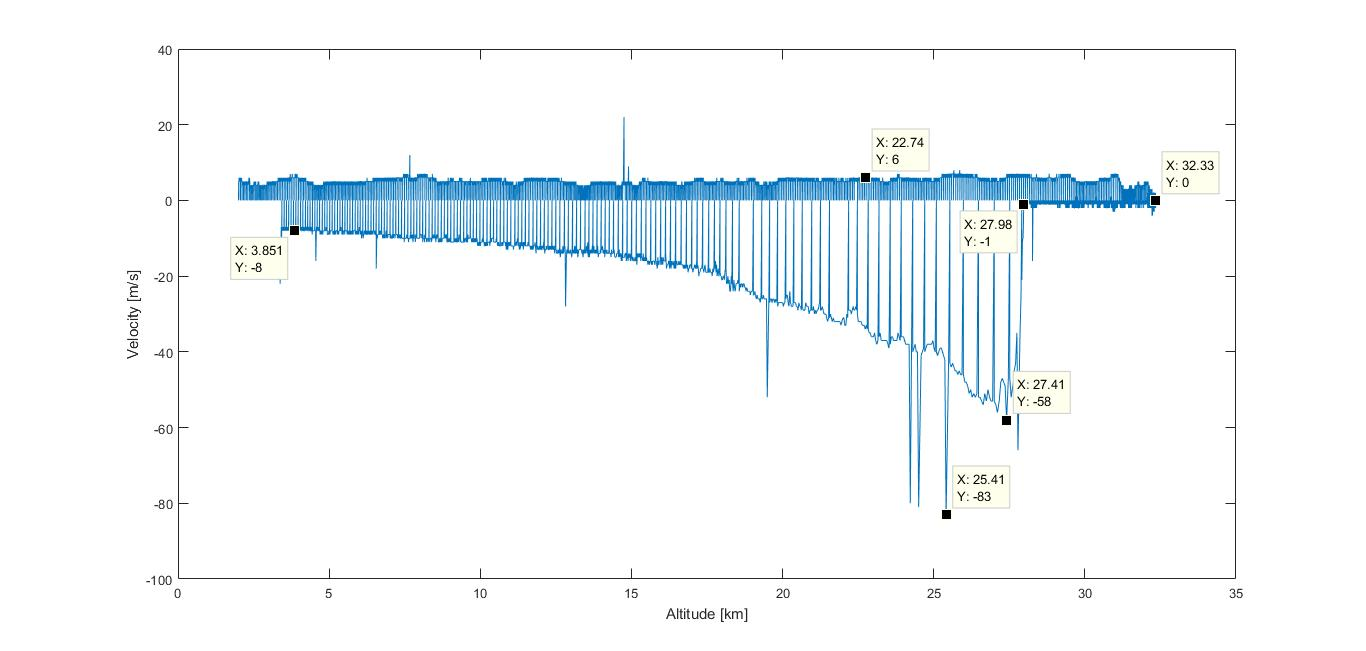
\includegraphics[width=1.2\textwidth]{appendix/img/velocity.png}}
    \end{align*}
    \caption{Vertical Velocity of the Gondola Over the Altitude During BEXUS 22 Flight}\label{fig:velocity}
\end{figure}

  

\bigskip
\underline{Atmospheric Conditions}

\smallskip
In order to see how the atmospheric conditions change during a BEXUS flight, the data from the BEXUS flight 22 was chosen for analysis. Figure \ref{fig:atmosphericconditions} below shows which kind of information is available for different parameters such as the temperature, the pressure and the air density with altitude.

\begin{figure}[H]
    \begin{align*}
    \noindent\makebox[\textwidth]{%
        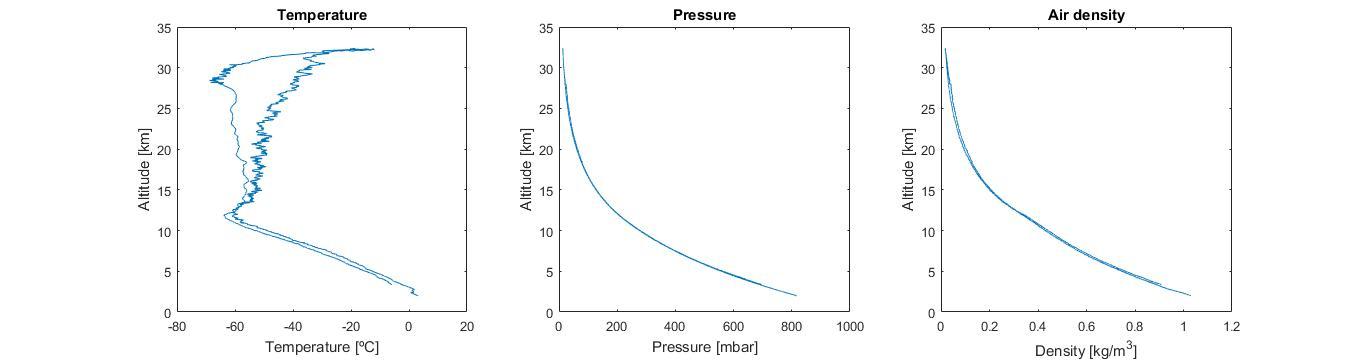
\includegraphics[width=1.3\textwidth]{appendix/img/atmospheric_variables.png}}
    \end{align*}
    \caption{Variations In Temperature, Pressure and Air Density During the Ascent and Descent Phase  for BEXUS flight 22}\label{fig:atmosphericconditions}
\end{figure}


\subsubsection{Trace Gases Distribution}\label{tracegases}

Atmospheric greenhouse gases are mostly concentrated in the upper troposphere and lower stratosphere. The Arctic region is of significant importance since there is where the maximum concentration of greenhouse gases is found due to meridional circulation (temperature differences) that pushes the gases from the equatorial to higher latitudes. Figures \ref{fig:carbondistribution} and \ref{fig:methanedistribution} are showing the concentration over latitude of two of the main greenhouse gases, $CO_2$ and $CH_4$ respectively.

\begin{figure}[H]
    \begin{align*}
    \noindent\makebox[\textwidth]{%
        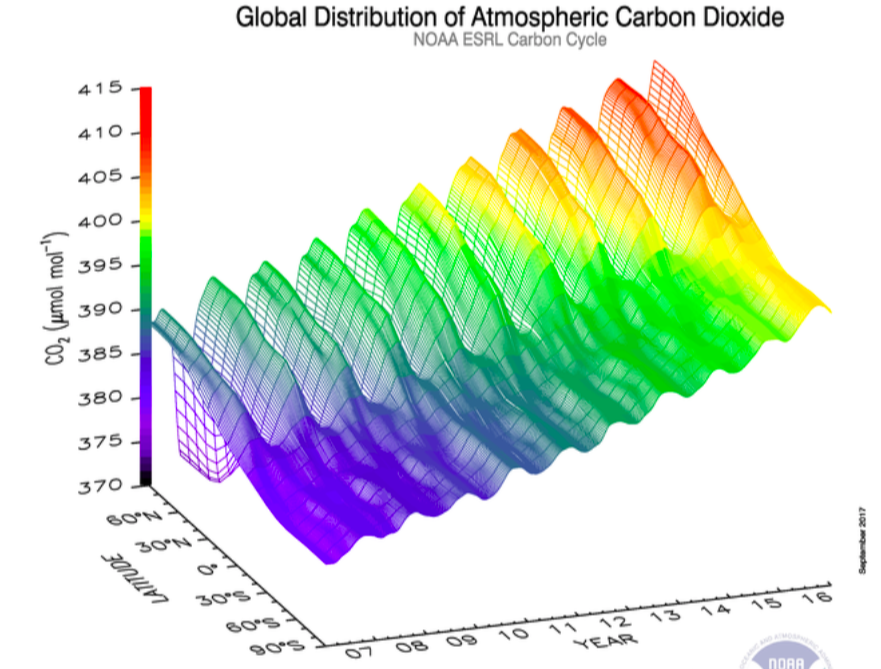
\includegraphics[width=0.8\textwidth]{appendix/img/carbondistribution.png}}
    \end{align*}
    \caption{Global Distribution of Atmospheric Carbon Dioxide\cite{latitude}}\label{fig:carbondistribution}
\end{figure}

\begin{figure}[H]
    \begin{align*}
    \noindent\makebox[\textwidth]{%
        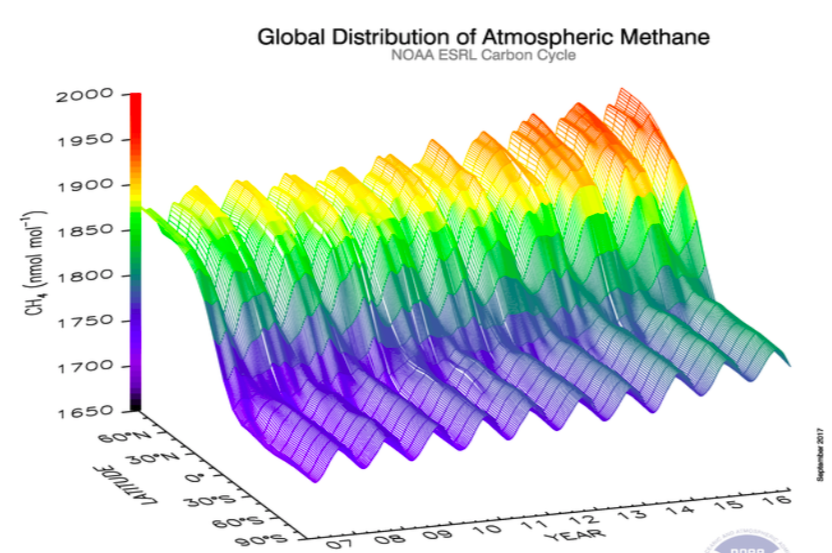
\includegraphics[width=0.8\textwidth]{appendix/img/methanedistribution.png}}
    \end{align*}
    \caption{Global Distribution of Atmospheric Methane\cite{latitude}}\label{fig:methanedistribution}
\end{figure}


The same applies for the vertical distribution of atmospheric greenhouse gases. The favoured altitudes for higher concentrations are the upper troposphere and the lower stratosphere due to gravity waves and the vertical wind, which carry the trace gases at higher altitudes. What is more, $CO_2$ has longer lifetime in the troposphere and stratosphere, where it has essentially no sources or sinks since it is basically chemically inert in the free troposphere.

\smallskip
Figure \ref{fig:verticalco2} shows the global distribution of carbon dioxide in the upper troposphere-stratosphere, at 50-60\degree N for the time period 2000-2010. 

\smallskip
Figure \ref{fig:seasonal} shows the global distribution of the seasonal cycle of the monthly mean $CO_2$ (in ppmv) in the upper troposphere and the lower stratosphere for the even months of 2010 and the altitude range from 5-45 $Km$. 

\begin{figure}[H]
    \begin{align*}
    \makebox[\textwidth]{%
        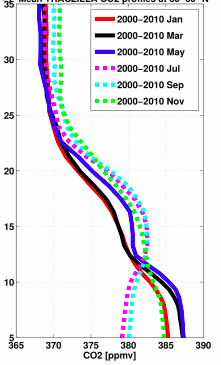
\includegraphics[width=0.4\textwidth]{appendix/img/verticaldistributionco2.png}}
    \end{align*}
    \caption{Global Distribution of $CO_2$ in the Upper Troposphere-Stratosphere\cite{CO2distribution}}\label{fig:verticalco2}
\end{figure}

\begin{figure}[H]
    \begin{align*}
    \noindent\makebox[\textwidth]{%
        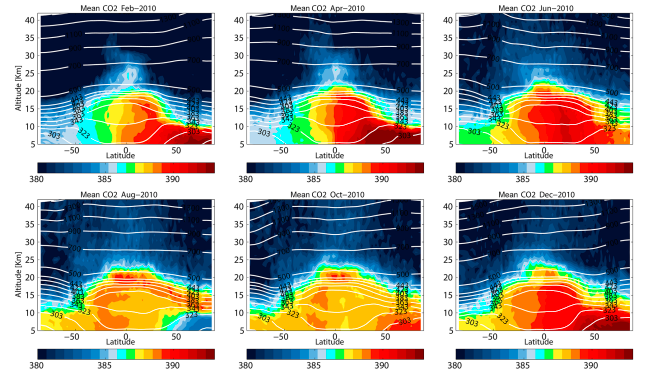
\includegraphics[width=1.2\textwidth]{appendix/img/monthlymeanc02.png}}
    \end{align*}
    \caption{Global Distribution of the Seasonal Cycle of the Monthly Mean $CO_2$ (in ppmv) in the Upper Troposphere and the Lower Stratosphere for the Even Months of 2010\cite{CO2distribution}}\label{fig:seasonal}
\end{figure}

Figures \ref{fig:verticalco2}, and \ref{fig:seasonal}, indicate that the higher $CO_2$ concentrations are found between 5 and 25 $km$ with peaks around 10 to 15 $km$ (figure \ref{fig:verticalco2}) and 20 $km$ for October (figure \ref{fig:seasonal}).

\smallskip
Figures \ref{fig:profile-olivier-membrive} and \ref{fig:profile-lisa} focus more on the region near the Arctic Circle. These figures represent vertical profiles distribution of $CO$, $CO_2$ and $CH_4$ extracted from past research papers \cite{LISA} \cite{Membrive}. The range of altitudes that will be compared is the one between 10 and 25 km. Since Figure \ref{fig:profile-olivier-membrive} vertical axis is in pressure, the equivalent pressures for these altitudes will be from approximately 200 hPa to 20 hPa. 

\begin{itemize}
    \item $CH_4$ distribution: There is a good agreement between both researches that the concentration around 10 km of altitude is about 1800 ppb and then it starts decreasing gradually with altitude. This decrease seems to be faster above 17 km (~70 hPa) which would make this the region of major interest. 
    \item $CO_2$ distribution: The concentration around 10 km is approximately 390-400 ppm in both researches. The biggest variation in concentration can be found between 10-17 km. The concentration of $CO_2$ seems to have an increase and then decrease again so this would be the most interesting range to sample. 
    \item $CO$ distribution: Only one research with CO profiles has been presented here so it cannot be compared with other researches. Analysing the only CO profile, it seems that the largest variation lays on the range 10-15 km, which should be the area of interest. 
\end{itemize}

Based on the vertical distribution profiles obtained from past researches, seems that our experiment should focus on sampling between 10-15 km for $CO$ and $CO_2$ but above 17 km for $CH_4$. 
\begin{figure}[H]
    \begin{align*}
    \noindent\makebox[\textwidth]{%
        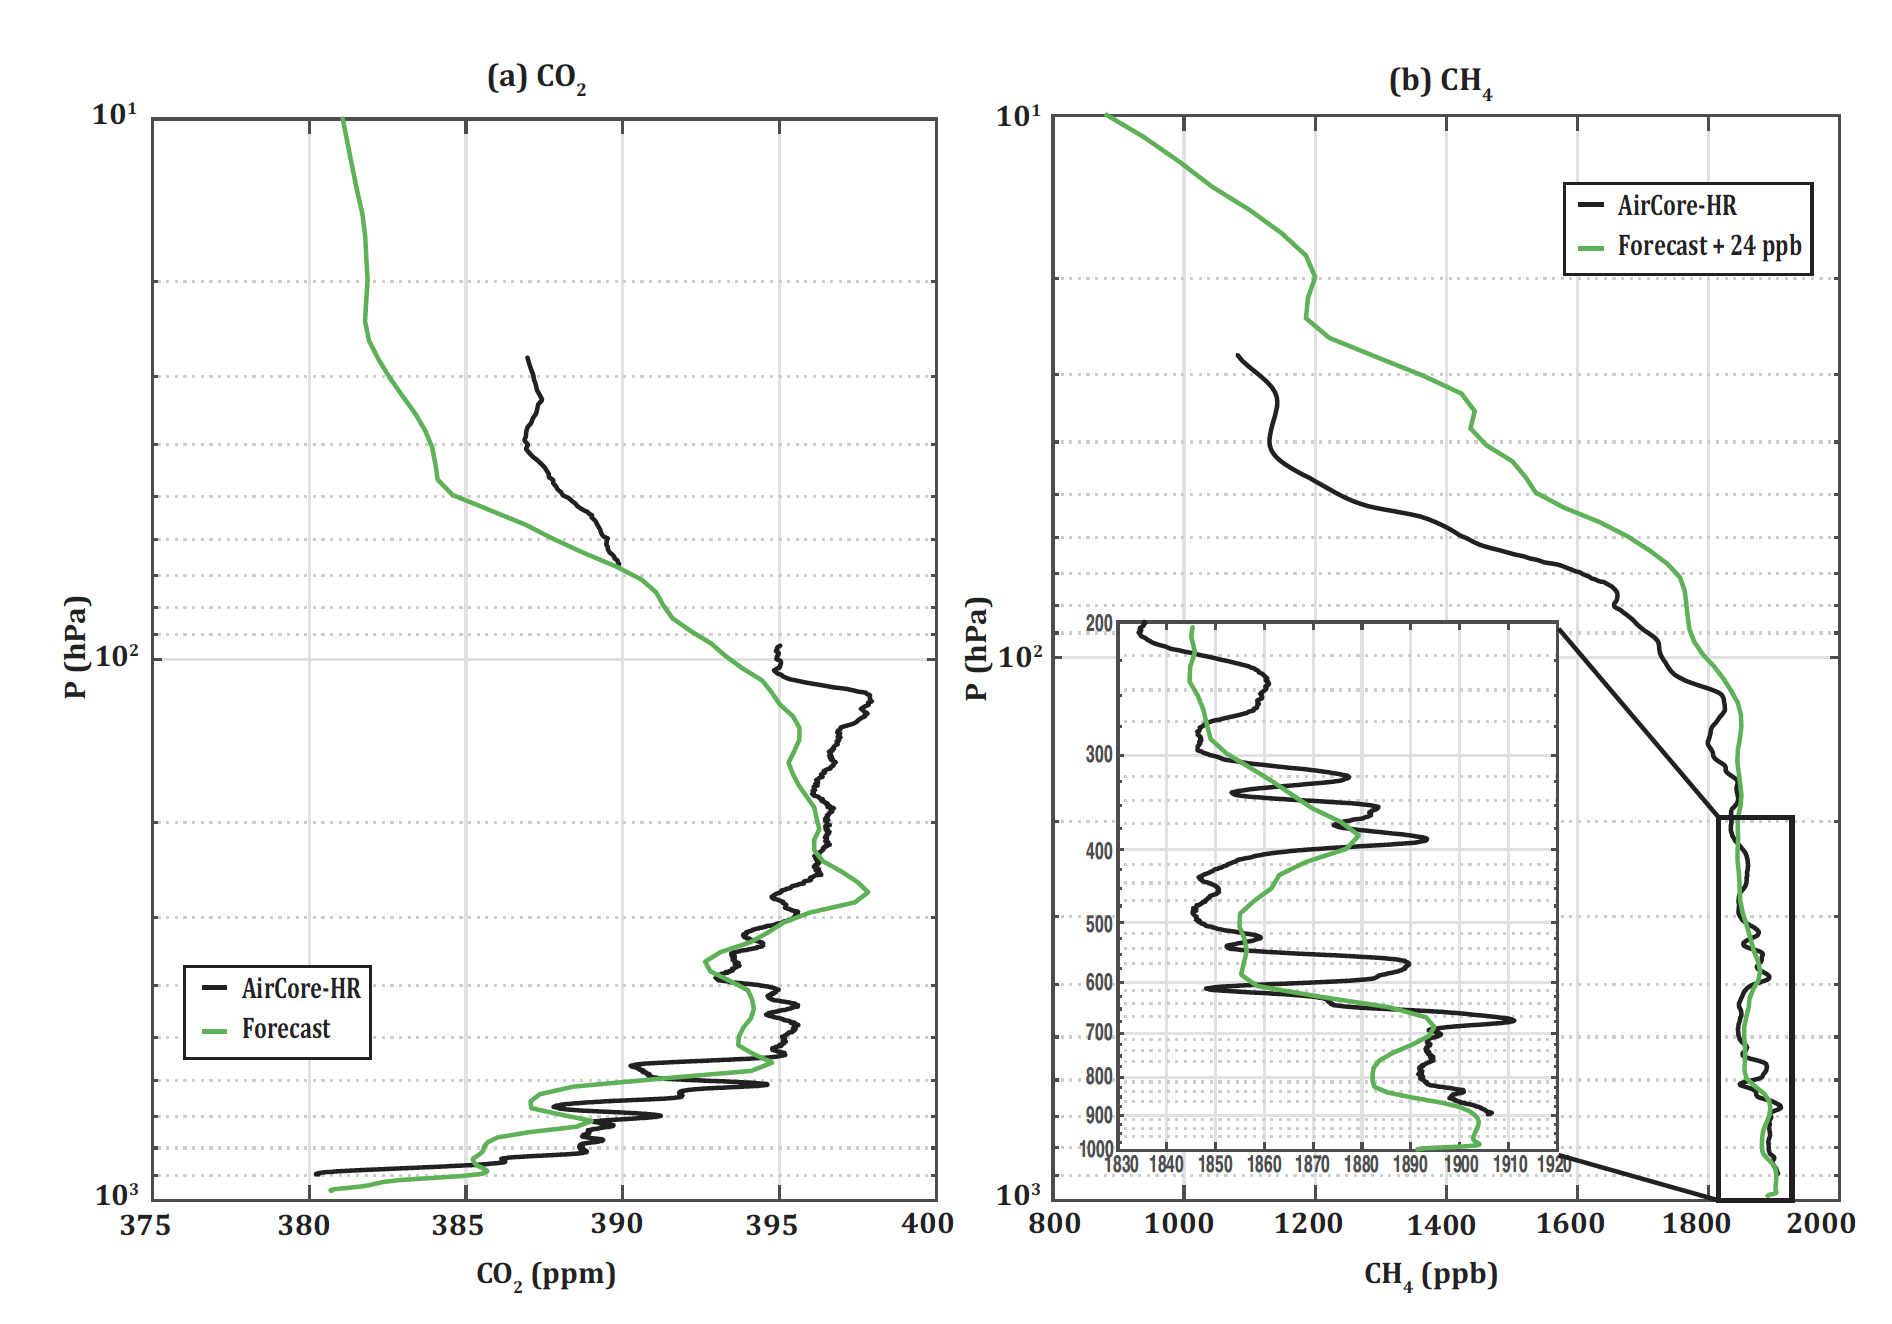
\includegraphics[width=1.1\textwidth]{appendix/img/profile-olivier-membrive.png}}
    \end{align*}
    \caption{Vertical Profiles in Black for $CO_2$ and $CH_4$. The Green Lines are High Resolution Forecasts \cite{Membrive}}\label{fig:profile-olivier-membrive}
\end{figure}

\begin{figure}[H]
    \begin{align*}
    \noindent\makebox[\textwidth]{%
        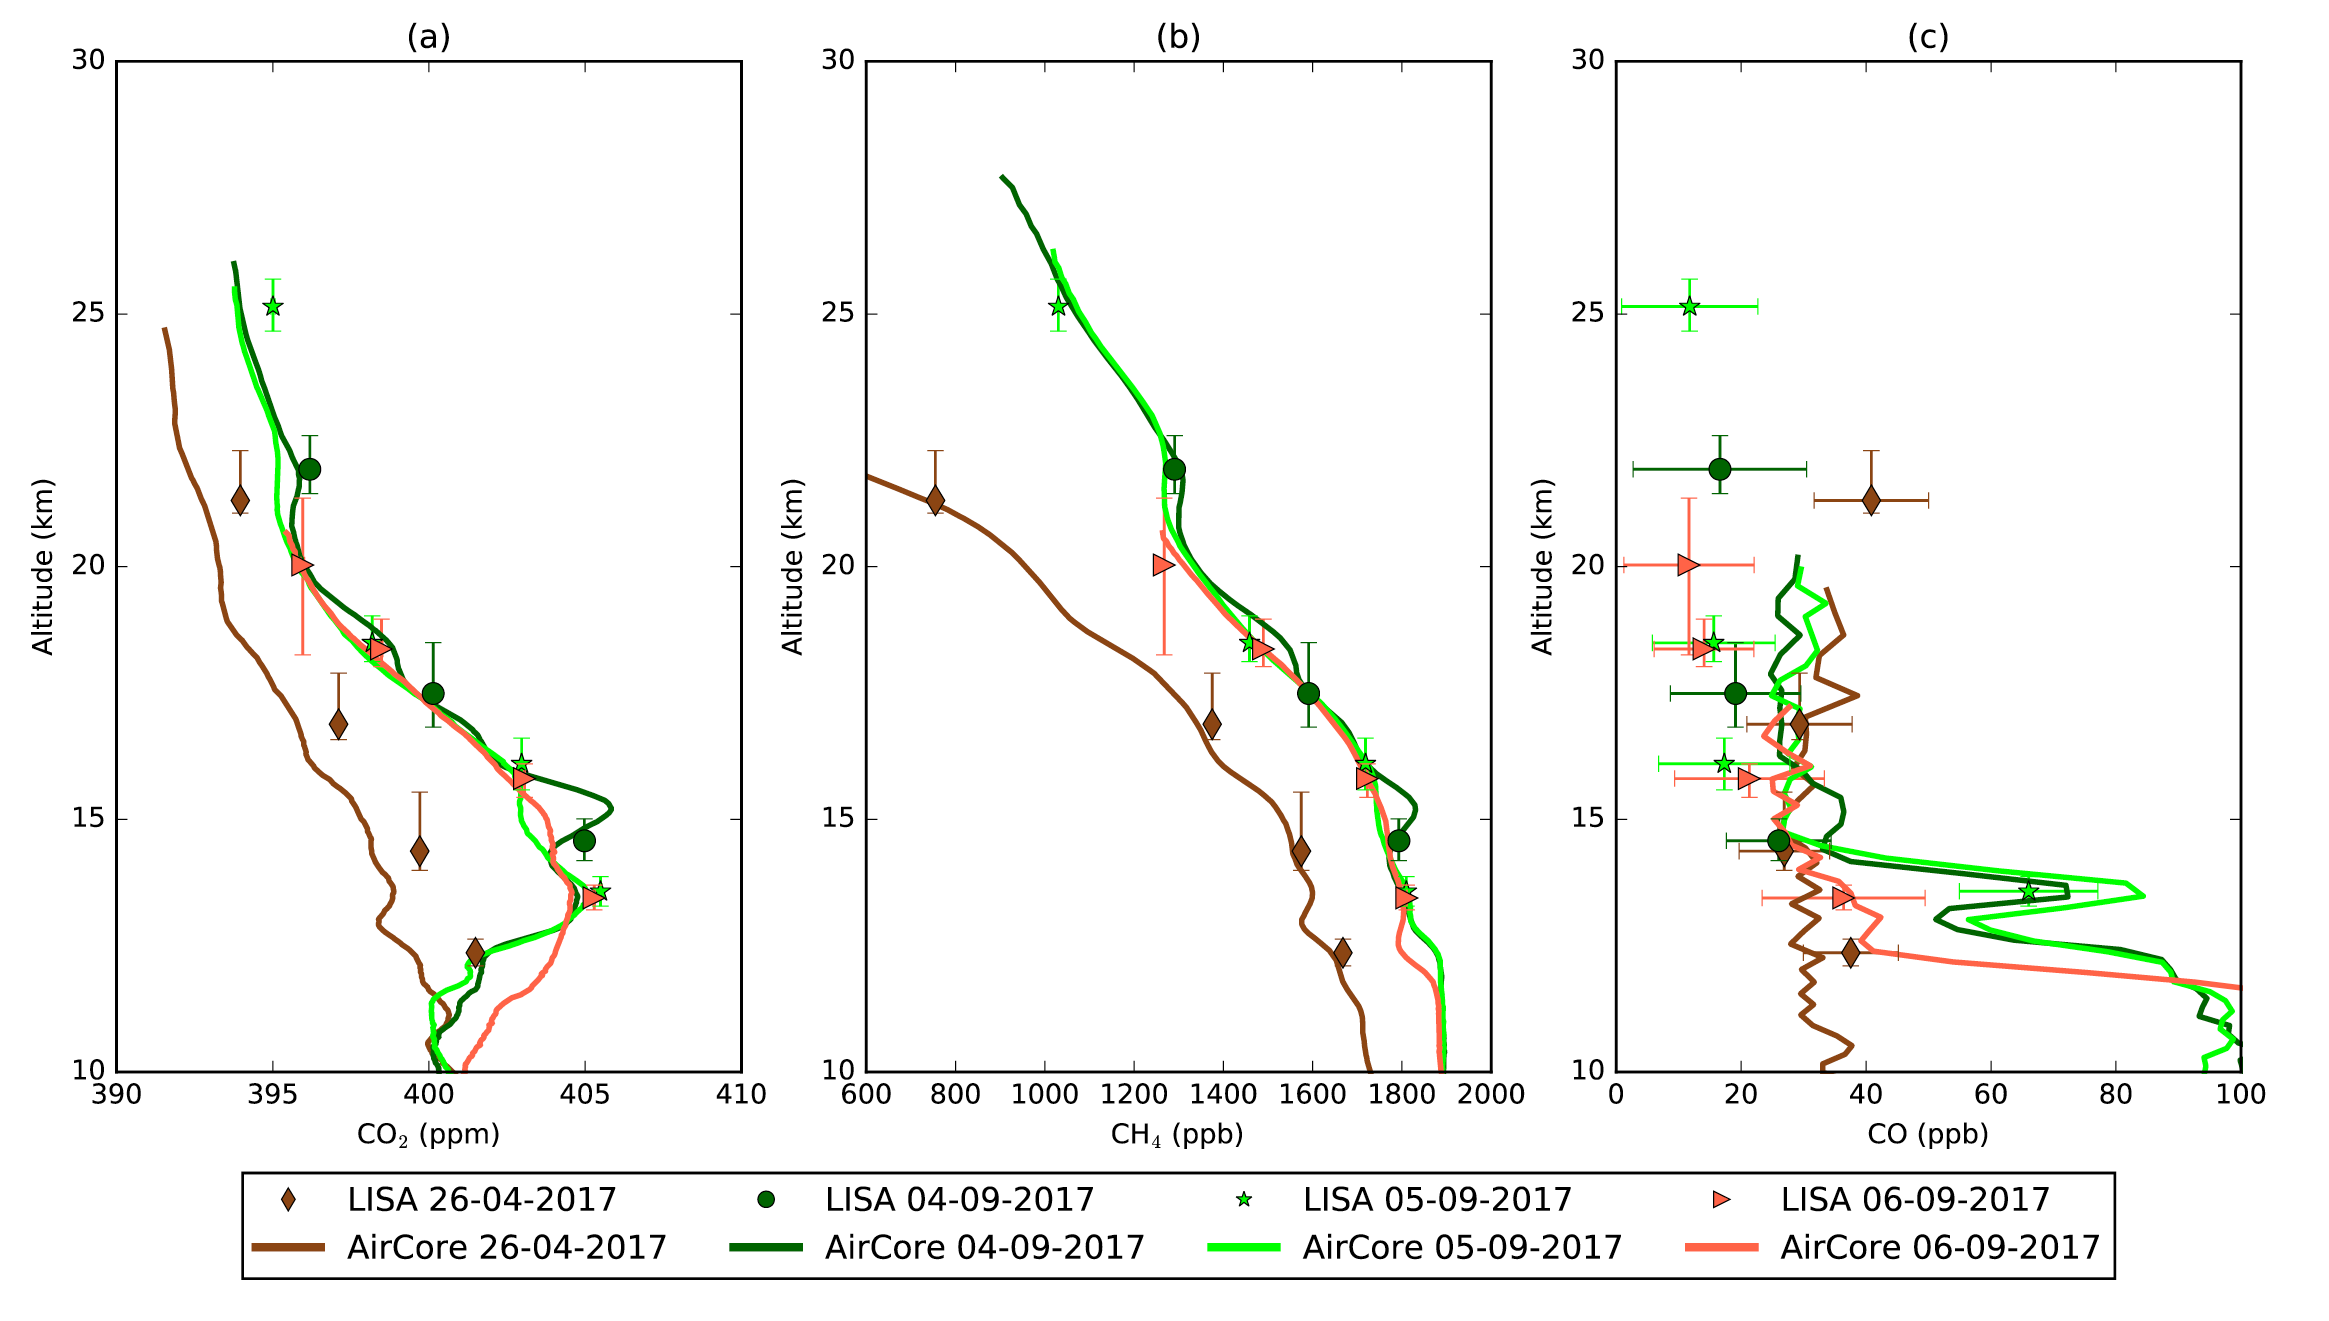
\includegraphics[width=1\textwidth]{appendix/img/profile-lisa.png}}
    \end{align*}
    \caption{Vertical Profiles Comparison of AirCore and LISA Measurements of $CO_2$, $CH_4$ and CO Mole Fractions  \cite{LISA}}\label{fig:profile-lisa}
\end{figure}


\subsection{Sampling Flowrate}
% \subsubsection{Pressure-Drop Flowrate}

%Air viscosity at ambient temperature (25ºC) and atmospheric pressure (1 atm = 101325 Pa) is about $10^-5$. This value decreases with the temperature and also with the pressure, which means that it is negligible in Artic conditions provided by Esrange location and specially in high altitudes. 

\subsubsection{Pump efficiency}

For the air sampling process, the micro diaphragm gas pum \emph{850 1.2 KNDC B} from KNFUSA company will be used.

By now, the team has already tested this pump in vacuum conditions in IRF facilities in Kiruna. Since the set of sensors required to obtain extra data such as the air flow rate, the pressure inside the bags and so on is not ready, the corresponding data is missing in Table \ref{tab:pump-flowrate-efficiency}. However, it has been proved that the pump is operative down to $20 mbar$.

\begin{table}[H]

\noindent\makebox[\columnwidth]{%
\scalebox{0.8}{
\begin{tabular}{|c|c|c|c|c|c|c|c|}
\hline
\textbf{Altitude} & \textbf{Pressure} & \textbf{Datasheet Flowrate} & \textbf{Datasheet Efficiency} & \textbf{Empirical Flowrate} & \textbf{Empirical Efficiency} \\ \hline
0\ km & 1013 mbar & 8 L/min & 100 \% &  &  \\ \hline
0.5\ km & 925 mbar & 7 L/min & 87.5 \% &  &  \\ \hline
1.5\ km & 850 mbar & 6 L/min & 75 \% &  &  \\ \hline
2.3\ km & 760 mbar & 5 L/min & 62.5 \% &  &  \\ \hline
3.1\ km & 680 mbar & 4 L/min & 50 \% &  &  \\ \hline
4.6\ km & 560 mbar & 3 L/min & 37.5 \% &  &  \\ \hline
6.4\ km & 450 mbar & 2 L/min & 25 \% &  &  \\ \hline
8.3\ km & 320 mbar & 1 L/min & 12.5 \% &  &  \\ \hline
10.7\ km & 230 mbar & 0 L/min & 0 \% & 4.865 L/min &  \\ \hline
12\ km & 194 mbar & 0 L/min & 0 \% &  &  \\ \hline
17\ km & 88 mbar & 0 L/min & 0 \% & 3.4 L/min &  \\ \hline
20\ km & 55.29 mbar & 0 L/min & 0 \% &  &  \\ \hline
24\ km & 30 mbar & 0 L/min & 0 \% & 3 L/min &  \\ \hline
30\ km & 11.97 mbar & 0 L/min & 0 \% &  &  \\ \hline

\end{tabular}}}

\caption{Pump Flowrate/Efficiency According to the Datasheet and Tests}
\label{tab:pump-flowrate-efficiency}
\end{table}

\subsection{Sampling strategy tests}

\subsubsection{Past research sampling strategy test}
Some of the most important parameters to be determined in this experiment are vertical resolution, sample size, sampling time and sampling flow rate amongst others. The difficulty in determining them lies on the fact that they are all interrelated. For example, the vertical resolution depends on the vertical speed and the effective sampling time. The amount of air samples that can be collected in each sampling bag is a function of the sampling time and the sampling flow rate. This is the reason why testing the pump's performance will be helpful to make a decision.

\smallskip
The test that will be realized is based on previous research \cite{LISA}. The tested elements will be the pump, one sampling bag, the outlet valve and the electronics necessary to record data (pressure and temperature sensors, datalogger and batteries). The simplified version of the experiment is placed in a vessel where the pressure can be regulated by a vacuum pump in order to simulate the desired atmospheric pressures.

\smallskip
The procedure for the test will be as follows: reach the desired pressure in the chamber and then start sampling air for 153 seconds. Repeat this process for three different pressures: 31.5 hPa, 60.8 hPa and 117.7 hPa. The data for pressure and temperature is logged at 3 Hz. The result of this measurements is represented in Figure \ref{fig:sampling-time-volume}. 

\begin{figure}[H]
    \begin{align*}
    \noindent\makebox[\textwidth]{%
        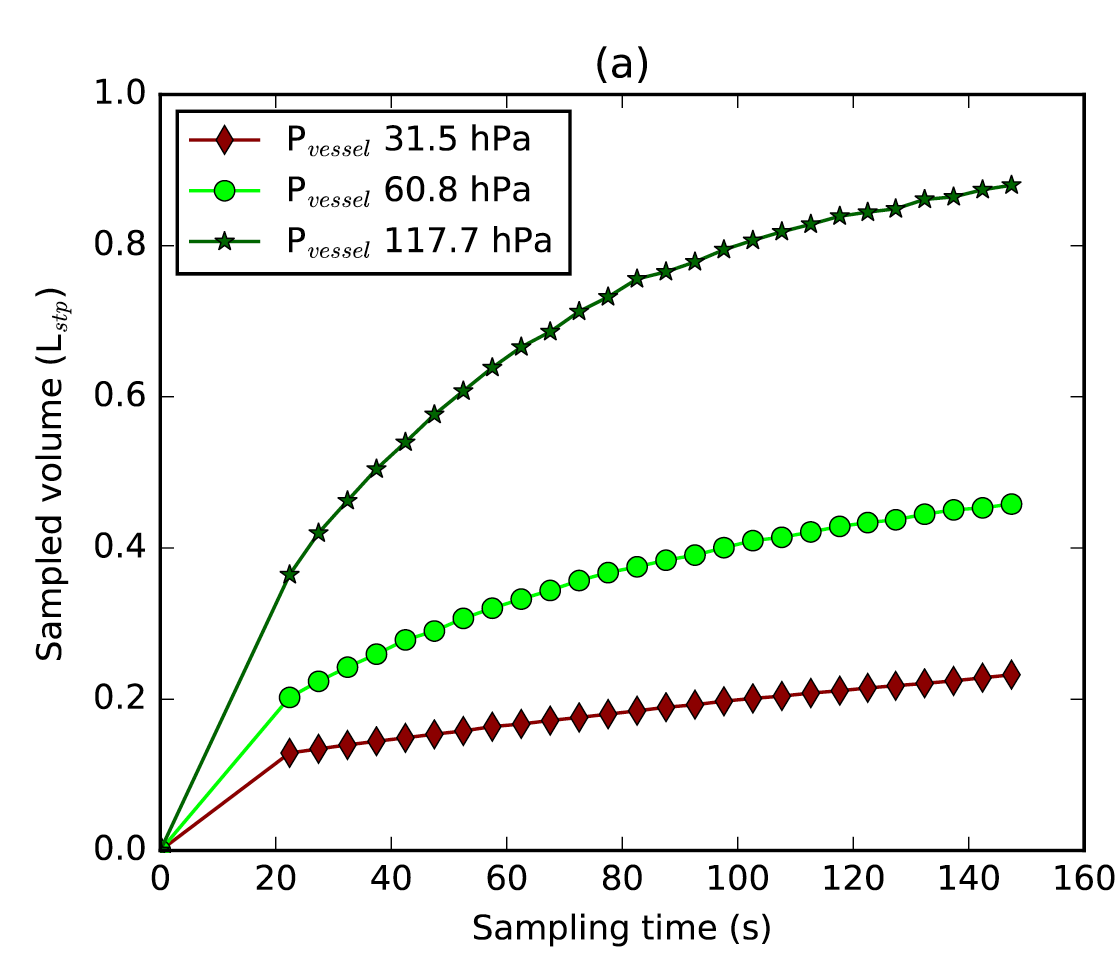
\includegraphics[width=0.7\textwidth]{appendix/img/sampling-time-volume.png}}
    \end{align*}
    \caption{Sampling Time (s) - Sampled Volume (L at STP)  \cite{LISA}}\label{fig:sampling-time-volume}
\end{figure}

As it can be seen in Figure \ref{fig:sampling-time-volume}, there is a lineal increase of the volume that corresponds to the first twenty seconds when the bag is expanding to its full size. Until then the pressure readings are constant but after that point is reached, the pressure inside the sampling bag starts to increase due to air compression. All the data points are calculated using the data logged from the sensors and the ideal gas law.

\smallskip
The next step is to use a non-linear least squares method to obtain an empirical model of the parameter named a(t) which is relating the volume at STP with the chamber pressure by the equation $V_{STP}=a(t)\cdot p_a$. The model is only valid for $t>19.7$ seconds which means that the sampling bag has reached total expansion. The fitted values for a(t) are represented in Figure \ref{fig:least-squares-a-fitting}. Once a(t) is obtained, Figure \ref{fig:vessel-p-volume} can be represented just to see the relationship between the vessel pressure and the sampled volume. Three arbitrary sampling times are chosen for this representation and an horizontal line represents the maximum pressure that the sampling bag can withstand. This implies another procedure during the test: fill the bag until the sealing breaks and calculate the differential pressure that was achieved between the inside and the outside.  

\begin{figure}[H]
    \begin{align*}
    \noindent\makebox[\textwidth]{%
        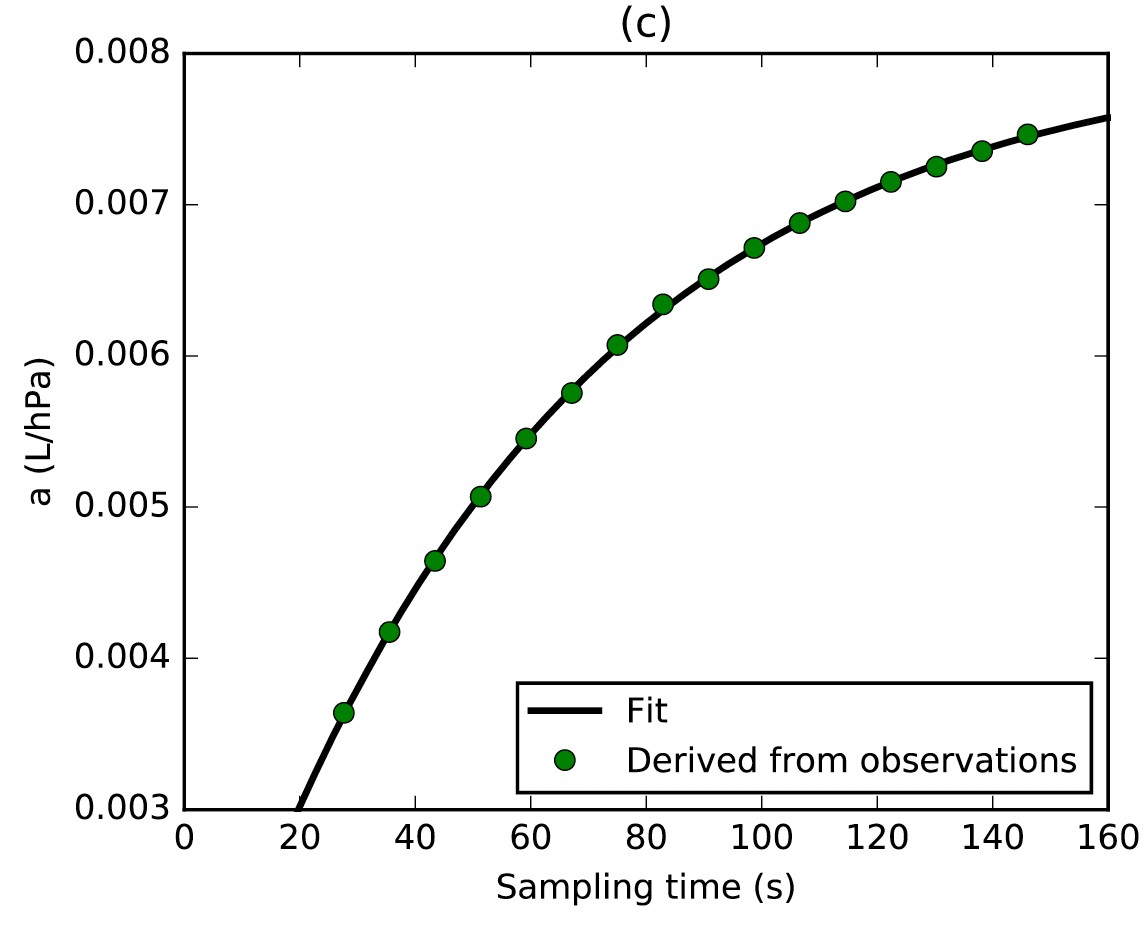
\includegraphics[width=0.7\textwidth]{appendix/img/least-squares-a-fitting.png}}
    \end{align*}
    \caption{Sampling Time (s) - a (L/hPa)  \cite{LISA}}\label{fig:least-squares-a-fitting}
\end{figure}



\begin{figure}[H]
    \begin{align*}
    \noindent\makebox[\textwidth]{%
        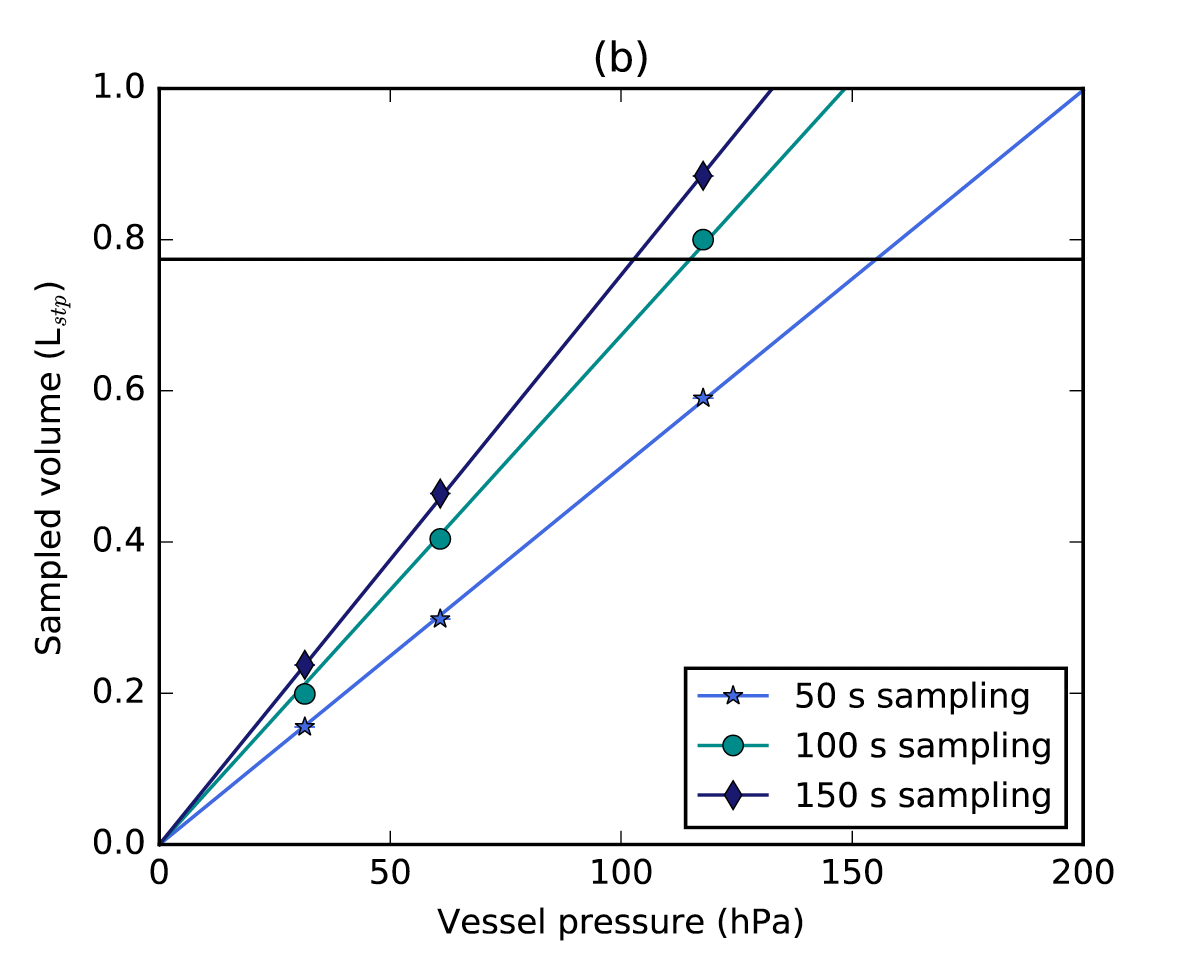
\includegraphics[width=0.7\textwidth]{appendix/img/vessel-p-volume.png}}
    \end{align*}
    \caption{Vessel Pressure (hPa) - Sampled Volume (L at STP) \cite{LISA}}\label{fig:vessel-p-volume}
\end{figure}

The objective of the above explained test and the calculations that follow will be to obtain an empirical model that gives the sampled air volume as a function of time at any pressure level. This will be the tool to calculate vertical resolutions and expected sample size and it should be a graphic looking like the one in Figure \ref{fig:sampled-volume-atm-p}.


\begin{figure}[H]
    \begin{align*}
    \noindent\makebox[\textwidth]{%
        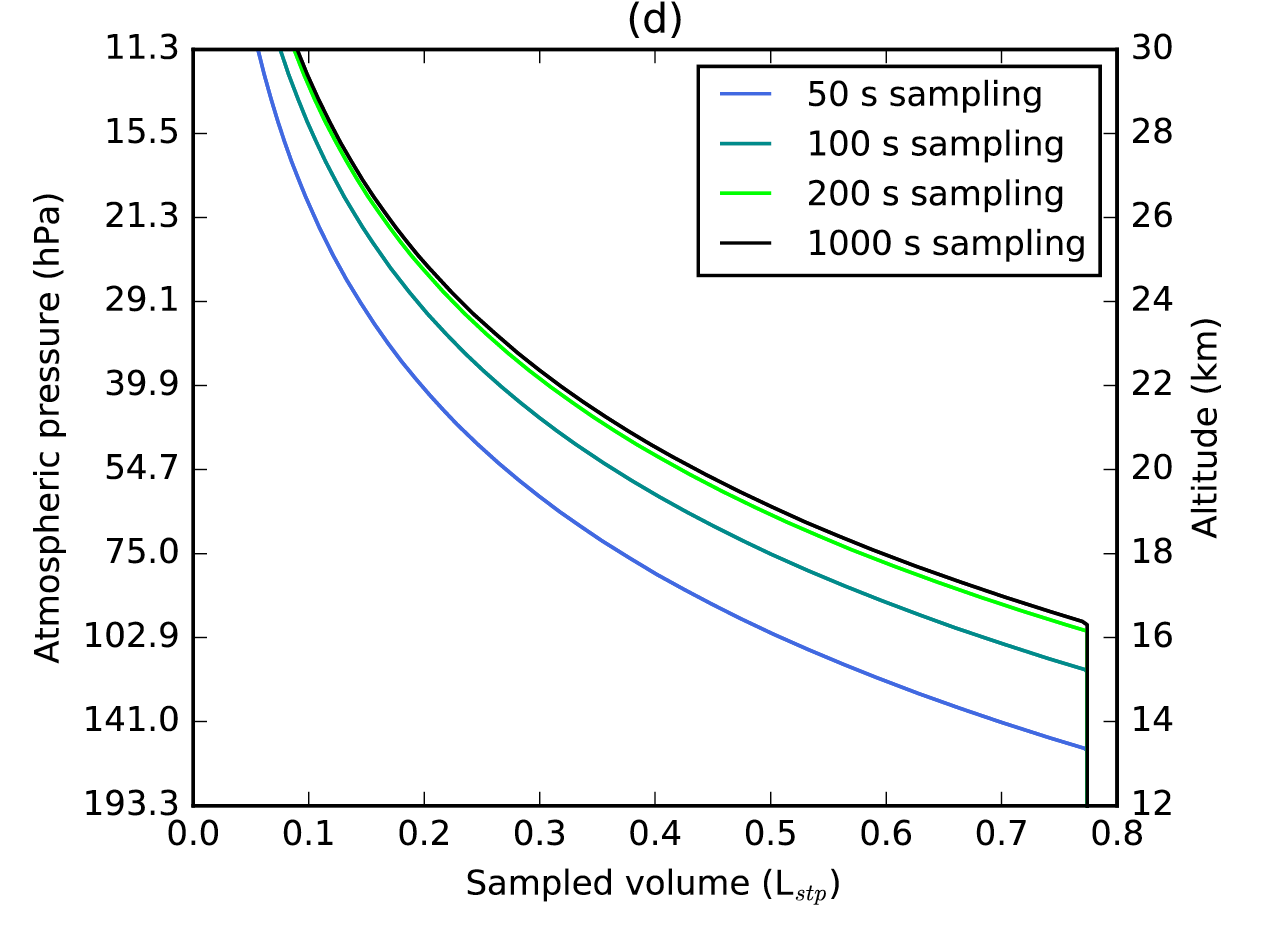
\includegraphics[width=0.7\textwidth]{appendix/img/sampled-volume-atm-p.png}}
    \end{align*}
    \caption{Sampled Volume (L at STP) - Atmospheric Pressure (hPa) \cite{LISA}}\label{fig:sampled-volume-atm-p}
\end{figure}

\subsubsection{Test results}
The above described test is Test 18 in Table \ref{tab:pump-low-pressure-test} the results of which can be found in section  \ref{subsection:pumplowpressuretest} 

% \subsection{Heat transfer}

\subsection{Discussion of the results}

\subsubsection{Computational methods vs. Flight measurements}
% Kalman filter (empiric data vs. mathematical model) Error estimation

\bigskip
\underline\subsubsubsection{Atmospheric Model}

%The International Standard Atmosphere (ISA) and the US Standard Atmosphere 1976 are pretty much in agreement with some differences in the temperature distribution at higher altitudes.
%In the International Standard Atmosphere model, air is assumed to be dry, clean and to have constant composition. The function limitation of this is that does not take into account humidity effects or differences in pressure due to wind.

\smallskip
In this section, the data from the past BEXUS flights is compared with the 1976 US Standard Atmosphere, for validation reasons. Figure \ref{fig:pressure22} compares the changes in pressure over altitude for the BEXUS flights with the atmospheric model. It can be seen that the flights data-sets are in good agreement with the atmospheric model. 

\begin{figure}[H]
    \begin{align*}
    \noindent\makebox[\textwidth]{%
        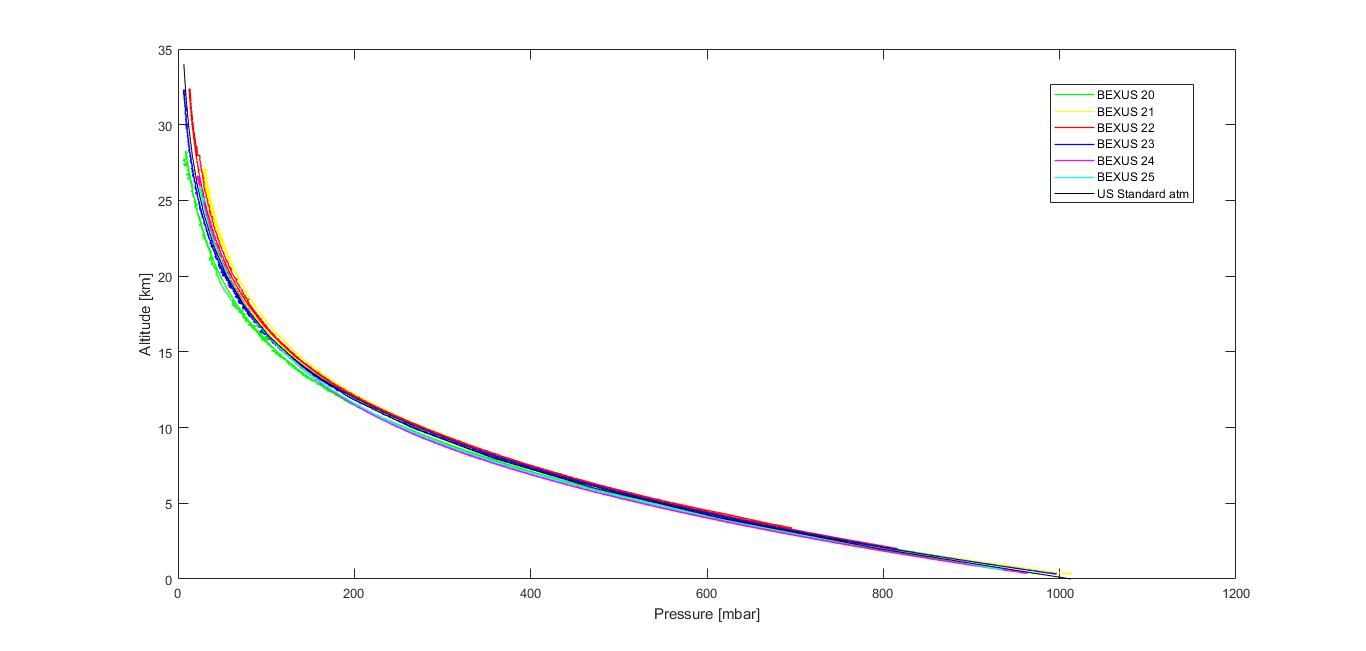
\includegraphics[width=1.3\textwidth]{appendix/img/pressureB22_USSA.png}}
    \end{align*}
    \caption{Comparative of Pressure Variation Over the Altitude During Different BEXUS Flights with the US Standard Atmosphere (1976)}\label{fig:pressure22}
\end{figure}

Figure \ref{fig:temperature22} below shows the changes in temperature over altitude, for all the BEXUS flights with the atmospheric model. It can be seen that there is a quite large deviation of the temperature above $20 km$ of altitude between the BEXUS flights and the US Standard Atmosphere 1976 model. This is not arbitrary since it appears in all flights. But it is not surprising either, because most of the atmospheric models fail to precisely predict the temperatures at higher altitudes.

\begin{figure}[H]
    \begin{align*}
    \noindent\makebox[\textwidth]{%
        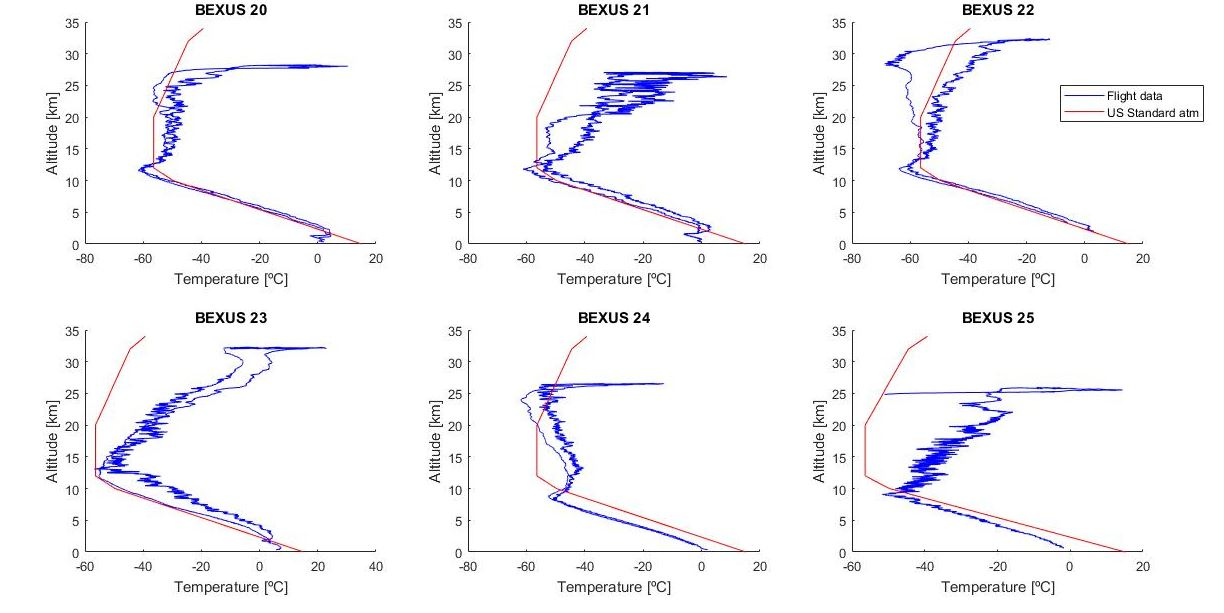
\includegraphics[width=1.2\textwidth]{appendix/img/allBX_z_T2.jpg}}
    \end{align*}
    \caption{Comparative of Temperature Variation Over the Altitude During Different BEXUS Flights with the US Standard Atmosphere (1976)}\label{fig:temperature22}
\end{figure}


\bigskip
\underlinesection{Descent Curve}

\smallskip
Again, in this section, the trajectories of past BEXUS flights, were compared with the mathematical model for validation reasons as shown in Figure \ref{fig:bexustrajectories}. Overall, BEXUS flights 20, 23 and 24 are in good agreement with the mathematical model. Some deviations exist between the mathematical model and the BEXUS flights 21 and 22 mostly in the last $5 km$ of the flight.    

\begin{figure}[H]
\noindent\makebox[\textwidth]{%
  \begin{subfigure}{0.45\textwidth}
    \centering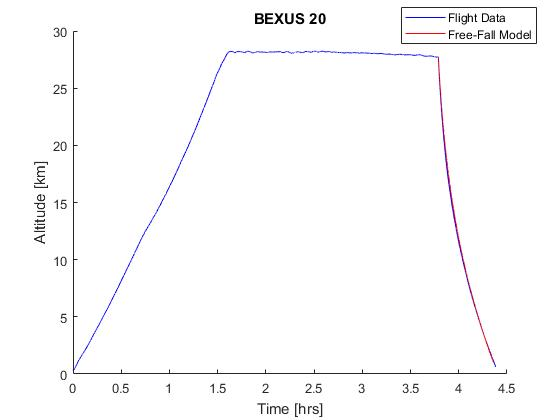
\includegraphics[width=1.1\textwidth]{appendix/img/bexus20mathmodel.png}
  \end{subfigure}
    \hfill
  \begin{subfigure}{0.45\textwidth}
    \centering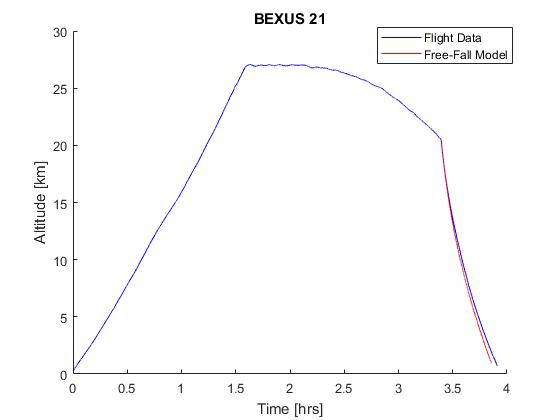
\includegraphics[width=1.1\textwidth]{appendix/img/bexus21mathmodel.png}
  \end{subfigure}}
  \noindent\makebox[\textwidth]{%
  \begin{subfigure}{0.45\textwidth}
    \centering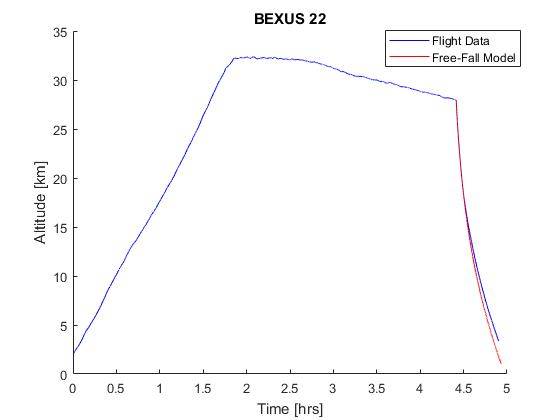
\includegraphics[width=1.1\textwidth]{appendix/img/bexus22mathmodel.png}
  \end{subfigure}
    \hfill
  \begin{subfigure}{0.45\textwidth}
    \centering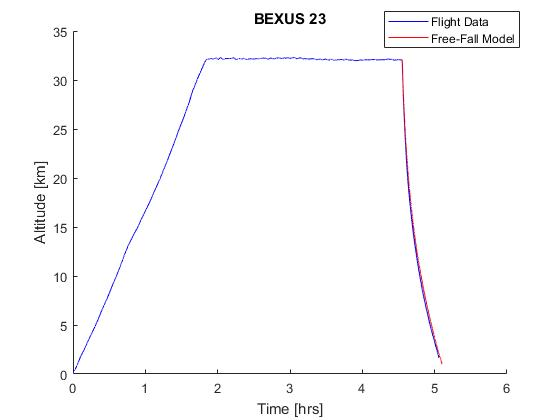
\includegraphics[width=1.1\textwidth]{appendix/img/bexus23mathmodel.png}
  \end{subfigure}}
  \centering
  \begin{subfigure}{0.45\textwidth}
    \centering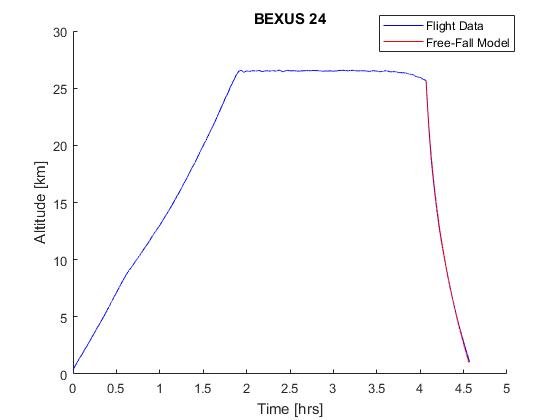
\includegraphics[width=1.1\textwidth]{appendix/img/bexus24mathmodel.png}
  \end{subfigure}
  \caption{Comparative of the Altitude Over Time During the BEXUS Flights 20, 21, 22, 23, 24 with the Mathematical Model}\label{fig:bexustrajectories}
  \end{figure}
  
 
 
\bigskip
\underlinesection{Velocity Profile}

\smallskip
Here, the mathematical model was compared with the velocity profiles during the flights. It can be seen that the mathematical model in general follows the velocity profile with some minor deviations during Descent Phase, which means that the estimation is quite reliable.

\begin{figure}[H]
\noindent\makebox[\textwidth]{%
  \begin{subfigure}{0.45\textwidth}
    \centering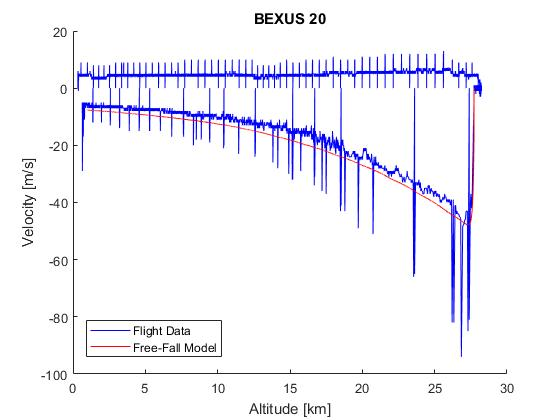
\includegraphics[width=8cm]{appendix/img/velocity20mathmodel.png}
  \end{subfigure}
  \hfill
  \begin{subfigure}{0.45\textwidth}
    \centering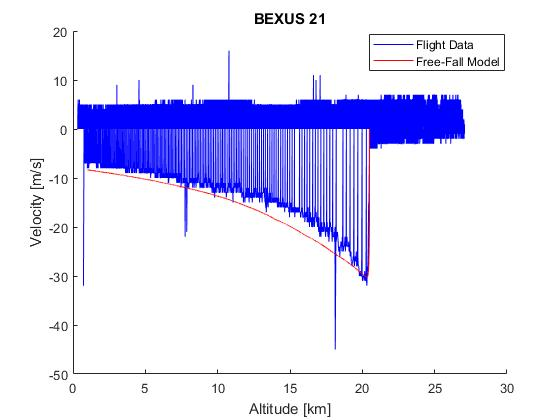
\includegraphics[width=8cm]{appendix/img/velocity21mathmodel.png}
  \end{subfigure}}
  \noindent\makebox[\textwidth]{%
  \begin{subfigure}{0.45\textwidth}
    \centering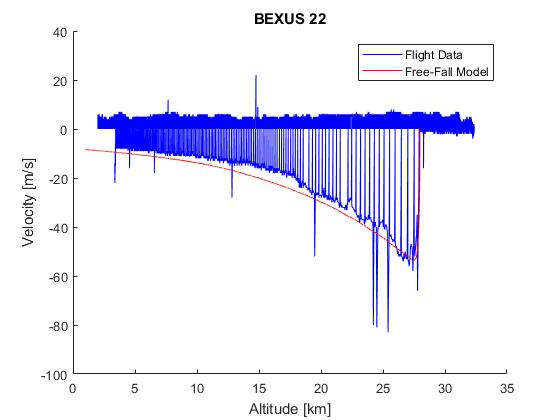
\includegraphics[width=8cm]{appendix/img/velocity22mathmodel.png}
  \end{subfigure}
  \hfill
  \begin{subfigure}{0.45\textwidth}
    \centering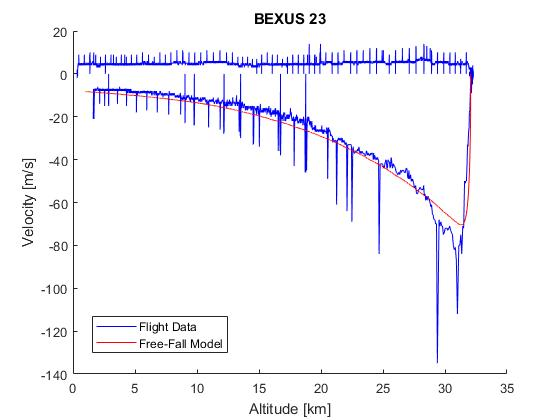
\includegraphics[width=8cm]{appendix/img/velocity23mathmodel.png}
  \end{subfigure}}
  \centering
  \begin{subfigure}{0.45\textwidth}
    \centering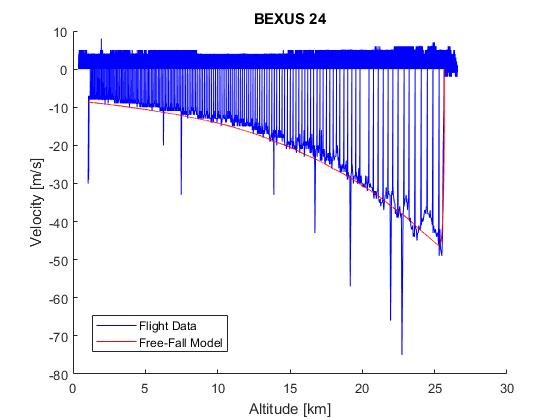
\includegraphics[width=8cm]{appendix/img/velocity24mathmodel.png}
  \end{subfigure}
  \caption{Comparative of the Velocity Over Altitude During the BEXUS Flights 20, 21, 22, 23, 24 with the Mathematical Model}
  \end{figure}
  


\subsubsection{Mass Effects in the Descent Curve}

Figure \ref{fig:masseffects}, shows how the descent time changes with different gondola mass values, after the cut-off phase. The heavier the payload, the sooner it will land. For example, if the gondola weights $250 kg$, it will land in approximately $25$ minutes after the cutoff, while it would take approximately $40$ minutes to land if it weights $100 kg$.   

\begin{figure}[H]
    \begin{align*}
    \noindent\makebox[\textwidth]{%
        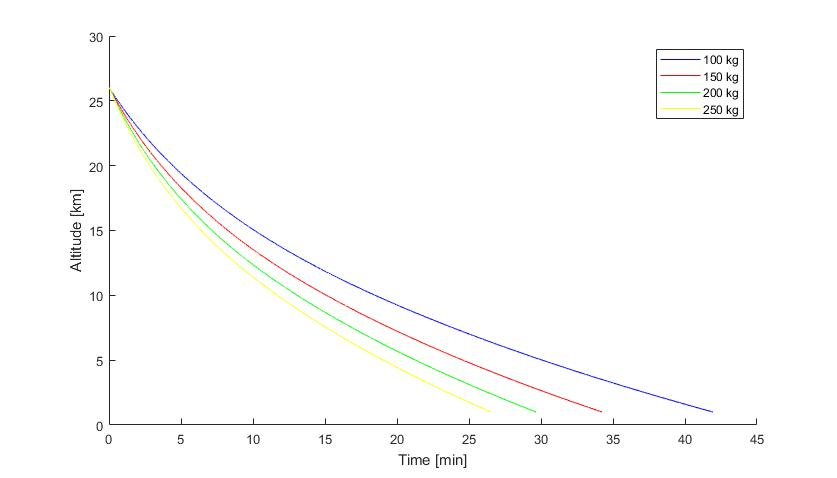
\includegraphics[width=1\textwidth]{appendix/img/masseffectsdescentcurve.png}}
    \end{align*}
    \caption{Mass Effects}\label{fig:masseffects}
\end{figure}


\subsubsection{Discrete Sampling Volumes}

Figure \ref{fig:samplingvolume} supports the team's decision to use a pump if sampling at high altitudes is meant, even though there is a single point failure risk. At $20 km$ of altitude, the minimum amount of air that would be needed to be sampled, in order to ensure that there is enough left for analysis at ground, would be almost $3 L$. Considering the low pressure at this high altitude, and the time it would be needed to fill the bag, it would be impossible to fulfill the experiment's objectives without using a pump. Moreover, without a pump, sampling at altitudes higher than $22 km$, and also during Ascent Phase, would be impossible.

\begin{figure}[H]
    \begin{align*}
    \noindent\makebox[\textwidth]{%
        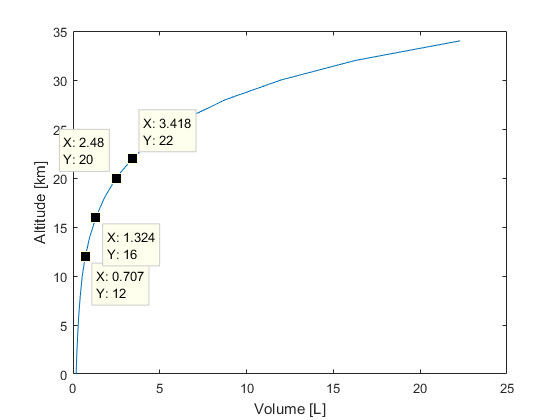
\includegraphics[width=1.2\textwidth]{appendix/img/new-data-points-13May.png}}
    \end{align*}
    \caption{Minimum Sampling Volume at Each Altitude to Obtain Enough Air to Perform a Proper Analysis (180 mL at sea level)}\label{fig:samplingvolume}
\end{figure}


\subsubsection{Limitations of the Bag Sampling Method}

\bigskip
\underlinesection{Roof Altitude Effect}

\smallskip
Since the pump's flow rate at high altitudes is not known yet, for a hypothetical study case, an ideal and continuous flow rate was used ($1 L/min$). The obtained diagrams below, show that even if the sampling starts at $26 km$, or at $30 km$, or at $40 km$, the number of filled bags would still be the same. This happens, due to the low pressure conditions at such altitudes which not allow a faster filling of a bag, and specially the low air density which forces to sample much more volume of air. Of course, the number of bags that can be filled, depends on the pump's efficiency at high altitudes.  So, the altitude of the gondola's cut-off over about $26 km$ would not affect the experiment's outcome. 

\begin{figure}[H]
\noindent\makebox[\textwidth]{%
  \begin{subfigure}{0.45\textwidth}
    \centering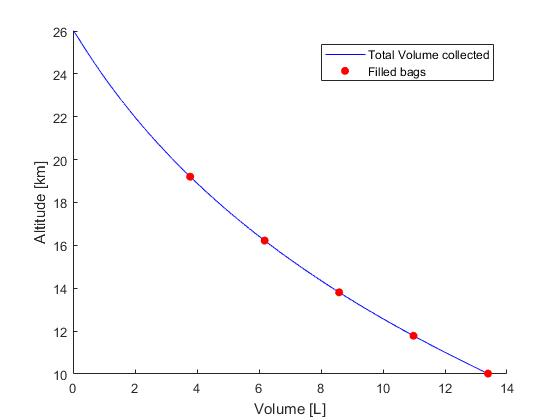
\includegraphics[width=1.2\textwidth]{appendix/img/samplevolume26km.png}
    \caption{Starting of Sampling at 26 $km$}
  \end{subfigure}
  \hfill
  \begin{subfigure}{0.45\textwidth}
    \centering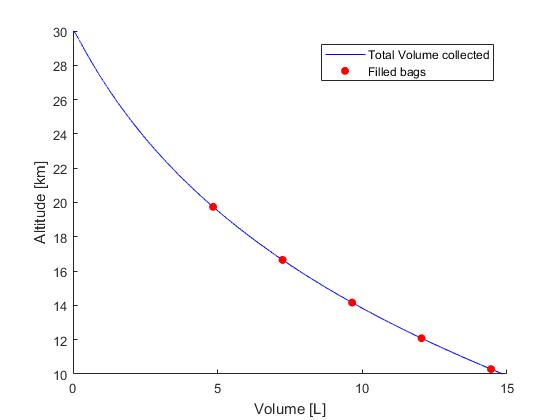
\includegraphics[width=1.2\textwidth]{appendix/img/samplevolume30km.png}
    \caption{Starting of Sampling at 30 $km$}
  \end{subfigure}}
  \centering
  \begin{subfigure}{0.45\textwidth}
    \centering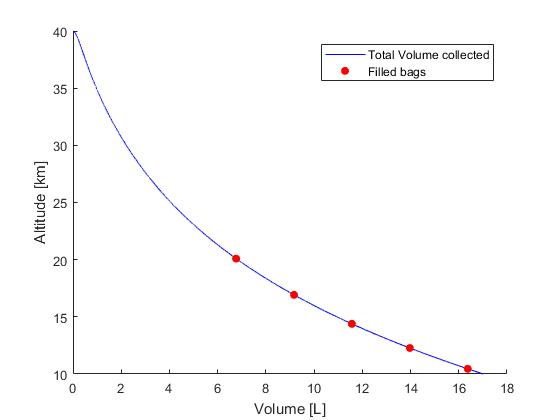
\includegraphics[width=1.2\textwidth]{appendix/img/samplevolume40km.png}
    \caption{Starting of Sampling at 40 $km$}
  \end{subfigure}
  \caption{Bag's Sampling System Limitations}\label{fig:limits}
\end{figure}
 

\bigskip
\underlinesection{One Single Pump}

\smallskip
Since the experiment uses a single pump, it is not possible to sample more than one bags at the same time. For the above hypothetical case, the maximum number of filled bags was five, considering continuous sampling. However, this is not the case when it comes to real life. Before sampling a bag, the system has to be flushed. Then, the sampling of a bag begins. After filling one bag, the system has to be flushed again before starting sampling a second bag. In that case, filling five bags, according to the hypothetical scenario, would be practically impossible.


\newpage
\subsection{Conclusions}
%\subsection{Reliability of the Simulation}
% strong points:
% weak points: Trace Gases Distribution

\subsubsection{Sampling Strategy}

After testing the pump at low pressure environment, an overall idea about the performance of the pump at high altitudes is now known and an approximation of the sampling strategy is possible.   
The total weight of the gondola is not known yet, but the balloon is expected to reach 25-27 km altitude, following the trajectory of the BEXUS 24 flight as shown in figure \ref{fig:bexustrajectories}. 
This serves the objectives of the TUBULAR experiment since, as indicated in section \ref{tracegases} the altitudes with higher differences in trace gases concentrations, are between 10 and 25 km. These are the altitudes where the sampling will be done. Sampling six bags in total, is enough to fulfil the objectives of the experiment and it is also feasible. Two bags will be sampled during Ascent Phase and four during Descent Phase. The ascent speed of the gondola, as shown in figure \ref{fig:altitudevelocity}, is estimated to be 6 m/s. A velocity of this rate, makes sampling of two bags possible while achieving a good resolution. It is important to mention here that the two bags that will be sampled during Ascent Phase, shall not be fully filled, since their volume will increase with decreasing pressure and may burst. For that reason, only about 80\% of their volume will be filled. On the other hand, during Descent Phase the four remaining bags shall be filled with the full 3 L. Since their volume will decrease with increasing pressure it has to be made sure that there will be enough sample left for analysis. 

The sampling of the first bag will start at 18 km of altitude. The sampling time is estimated to be 44s with an achieved resolution of 262m. The second bag will be sampled at 21 km of altitude, and it will take 47 s to fill the desired volume of air, with a resolution of 279 m. Before sampling, flushing of the AAC system for 1min is taking into account. During that, the gondola will cover a distance of 360 m. 

During Descent Phase, the sampling of the third will start from 17.5 km. The sampling time is estimated to be 52.94 sec with a resolution of 423.53 m. Bag no 4 will be sampled at 16 km for 50.0 s and resolution of 400 m. The fifth bag will be sampled at 14 km for 47.37 s and resolution of 378.95 m. The sample of the last bag will start at 12 km for 40.91 s sampling time and 327.27 m resolution. Again, one minute of flushing is taken into account, in between the sampling of each bag.

The flow rates of the pump, at each sampling altitude were taken from Figure \ref{fig:pump-performance}.




%Figure \ref{fig:samplingvolume} shows the minimum amount of air that needs to be sampled at each altitude in order to have enough left for analysis on ground. At 17 km the volume needed is approximately 2.5L. So, it would take 150 seconds and 900m to sample the first bag. Starting the sampling of the second bag at 18km, it would take 156sec and 936m to fill it with the minimum volume of air, approximately 2.6L. For the third bag, starting the sampling from 20 km it would take 168 second and 1.008 km to sample 2.8 L of air. The last bag would need 300 second and 1.8km to sample almost 5 L of air, starting from 22 km. In total, with one minute of flushing before each sampling of a bag, is 1014 seconds or 28 minutes.
%---------------------------------------------
\subsubsection{Discusion of the Results}
Overall, the mathematical model is in good agreement with the data from the past BEXUS flights as well as, with the atmospheric model used for the Arctic region.
Making this document, helped the team to cross-check some theoretical values, important for the layout and the planning of the experiment. Tables \ref{table:pre-flight} and \ref{table:post-flight} show that the estimated data before each flight are pretty close with the real data obtained by the flights which will help the team to define the experiment's parameters with higher accuracy. 
In order to make a sampling plan, it is important to know the duration time of each phase. Figure \ref{fig:trajectories}, shows the trajectories of the different BEXUS flights, giving the team a general idea of what the trajectory of the flight can look like and how the duration of each phase changes regarding the maximum altitude that the gondola reaches.

The velocity profile, figure \ref{fig:velocity}, is of high importance since the velocity during ascent and Descent Phase, will determine the resolution of the samples. In general, the velocity values are in agreement with the BEXUS manual, with an ascent speed of 6 m/s and a descent speed, fluctuating after cutoff, before stabilizing at 8 m/s at the last kilometers of the flight. Another important thing that has to be mentioned here, is the team's decision to sample during Ascent Phase too and not only during Descent Phase. As seen in figure \ref{fig:velocity} the gondola is turbulent after the cutoff with velocities up to 83 m/s, and needs more or less 6 km before stabilizing its velocity as figure \ref{fig:altitudevelocity} indicates. Hence, the altitudes that the gondola will be turbulent, will be covered by sampling during Ascent Phase. This will not affect the comparison with the CAC that will be sampled during Descent Phase only, since the horizontal displacement of the gondola is much smaller than the vertical. 

Atmospheric conditions play a crucial role for the TUBULAR experiment. The team should know, the different pressures at each altitude, since the pressure is the parameter that will trigger the sampling of the bags. What is more, the pressure will determine the performance of the pump and it is crucial to know under what pressures the pump needs to be tested depending on the sample altitude. The temperature is of high importance too and the trickier to predict especially at high altitudes. The team should be able to keep the temperature of the pump within its working temperature range in order to assure that the pump will start working. To do so, the air temperature must be known at each altitude which will help the team to come up with a good thermal plan. 

The sampling altitude range will not be chosen randomly. The idea is to find the altitude range, where the trace gases show the bigger differences in concentration. In section \ref{tracegases}, were presented some theoretical trace gases concentration values as well as, some results from past research papers. According to them, the more interesting area to sample is between 10 and 25 km of altitude. The team, plans to sample between 17 and 22 km during Ascent Phase and 17 to 10 km during Descent Phase. 

Additionally, the sampling software revealed some limitations of the sampling system and also which parameters should be taken into account for the experiment's layout and which not. 
The weight of the gondola, will affect the maximum altitude that the balloon will reach, and the time needed for the gondola to land, but it doesn't contribute to the decision of how many bags will be used.

The decision of the team to use a pump was questioned at the beginning, as a single point failure risk. However, this decision is justified by the need of sampling during Ascent Phase, ohterwise the sampling would not be possile.  Figure \ref{fig:samplingvolume}, supports the use of a pump because without a pump, sampling at 22 km of altitude, would be impossible considering the low pressure and the time it would take to fill a bag. 

Note that even with the pump, some limitations still exist. The sampling of the bags cannot be continuous since the system has to be flushed before sampling a bag. Furthermore, the flow rate of the pump will be lower at high altitudes than it is on the ground, due to pressure differences. Figure \ref{fig:limits} points out that even with an ideal flow rate of 1 L/min and sampling continuously, it is not possible to sample more than five bags, because it takes a lot of time to sample a bag at high altitude atmospheric conditions. Additionally, it makes clear why the maximum altitude that the gondola will reach, does not affect the experiment's outcome. As the gondola ascents, the pressure gets lower and takes more time to sample a bag. So, sampling more bags would not be possible even if the balloon reaches a higher altitude. The same applies for the Descent Phase and the cutoff altitude. 

Concluding, whilst at the beginning, the idea was to sample a total of sixteen bags in order to have more samples to compare with the continuous vertical profile obtained by the CAC, this document justifies that this is not feasible. Taking into account all the different parameters, it made clear which of them are important and which are not. Parameters like the gondola's velocity, the pressure at different altitudes, and the pump's flow rate, will determine the outcome of the TUBULAR experiment, the number of the bags that will be used, as well as the sampling altitudes. Parameters like the gondola's weight or the maximum altitude that the balloon will reach, does not affect the experiment's outcome and have a secondary role.


Note that after the pump tests, the sampling altitudes may change.   







\newpage